\documentclass[paper=b4, twocolumn, fleqn, fontsize=12pt, jafontscale=0.925, line_length=110mm, head_space=10mm, foot_space=10mm, dvipdfmx]{jlreq}
\setlength{\columnseprule}{0.4pt}
\pagestyle{empty}
\usepackage{bxpapersize}%用紙サイズ設定
\usepackage{tikz,ascmac,amsmath,amssymb,amsthm,bm,physics,arydshln,mathcomp,wrapfig,pgfplots,multicol,graphicx,fancybox}

\begin{document}

\twocolumn[%
	\begin{flushleft}
	  \LARGE\textbf{ワークシート　確率}
	\end{flushleft}
	\vspace{5mm}
	\begin{flushright}
		2年\underline{\hspace{3\zw}}組\underline{\hspace{3\zw}}番
		\hspace{1\zw}氏名\underline{\hspace{15\zw}}
	\end{flushright}
	\vspace{5mm}]
	
◎どちらの屋台が当たりやすい？

\textbf{ A : $100$ 本中 \ $30$ 本当たり}

\textbf{ B : $200$ 本中 \ $40$ 本当たり}

\begin{itembox}[l]{自分の考えを書いてみよう}
\vspace{4zw}
\end{itembox}

\vspace{5zw}

◎さいころで $1$ の目が出る確率 

\begin{figure}
  \centering
  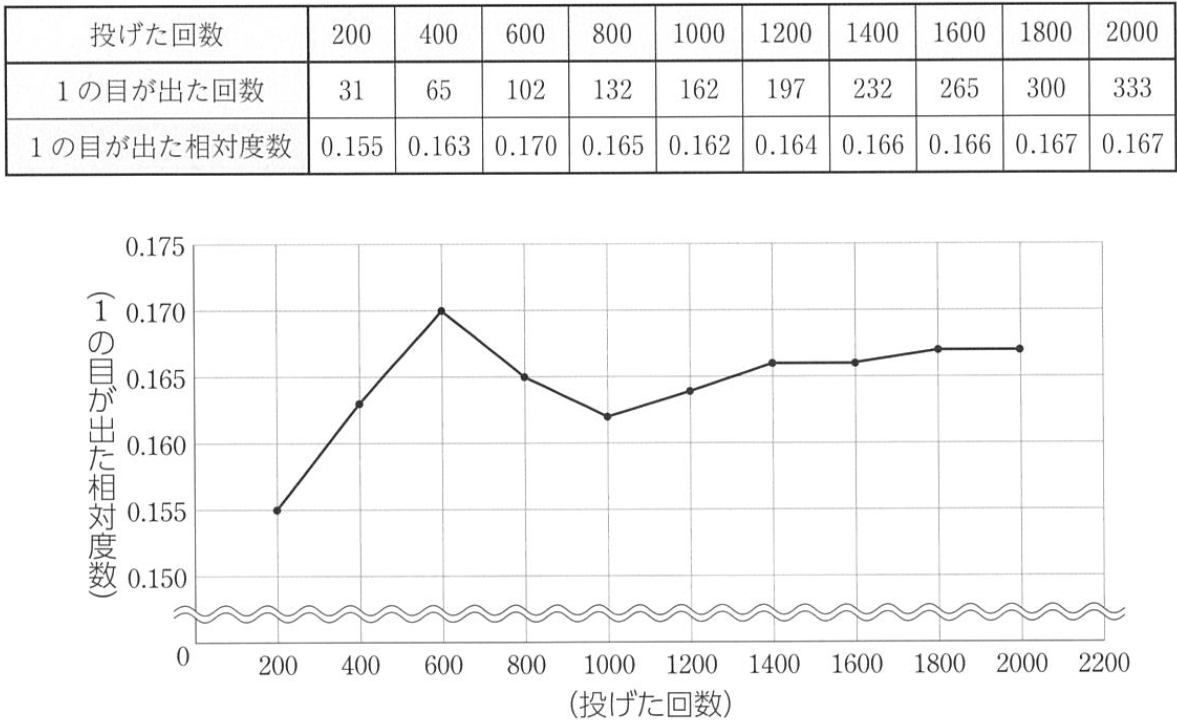
\includegraphics[height=18zw, width=28zw]{worksheetfigure.png}
\end{figure}

試行回数を増やすほど, \ 相対度数は一定の値

$0.167 \cdots = \displaystyle \frac{1}{6}$ に近づく.

\bigskip
\bigskip

これはほかの同じ目についても同じ相対度数が得られる.

$\Longrightarrow$ どの目が出ることも同じ程度に期待できる.

\bigskip

このとき, \ 各場合の起こることは 
\begin{flushright}
{\large\doublebox{　\hspace{8zw}}} %全角スペースを入れて調整 
という.  
\end{flushright}

\vspace{5zw}

\begin{itembox}[l]{メモ欄}
\vspace{15zw}
\end{itembox}

\newpage

\begin{figure}
  \centering
  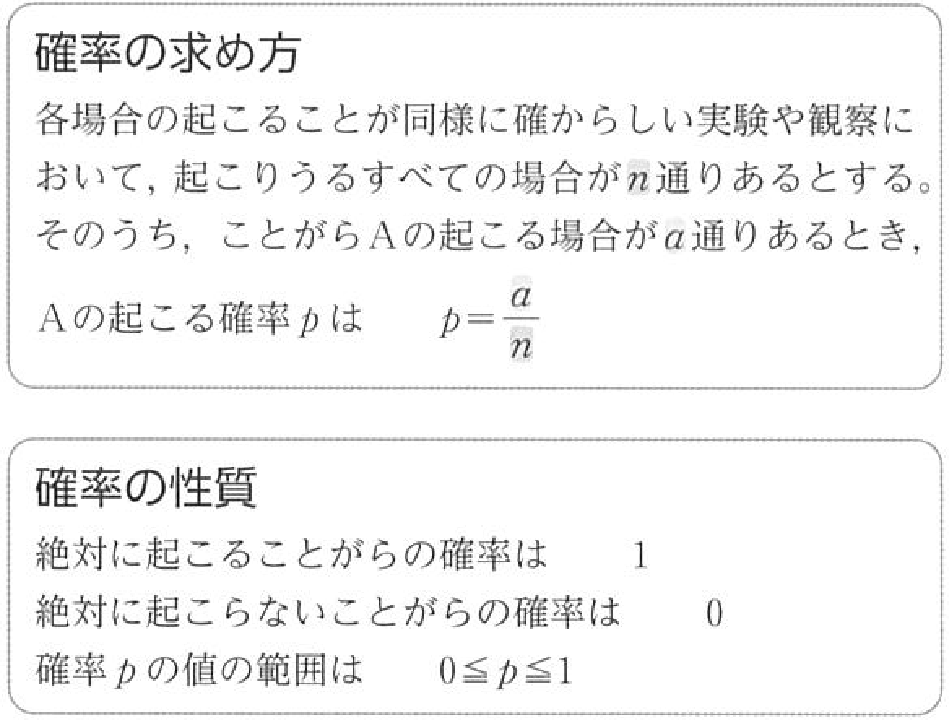
\includegraphics[height=20zw, width=28zw]{matome.png}
\end{figure}

\vspace{3zw}

\noindent
\textbf{例1 \ （硬貨の裏表の確率）}
  
$1$ 枚の硬貨を投げたとき, \ 表が出る確率を求めよう.

\bigskip

硬貨を投げたとき, \ 表と裏の出方は \fbox{　} 通りあり, \\
それらは\textgt{同様に確からしい}. そのうち, \ 表が出る場合は \fbox{　} 通りであるから, \ 表が出る確率は {\huge\fbox{　}}.

\bigskip

では, \ 裏が出る確率はどうだろうか? 表が出る確率と異なるだろうか.
（問１）

\vspace{5zw}

\noindent
\textbf{例2 \ （さいころの目の確率）}

$1$ 個のさいころを投げるとき, \ $3$ の倍数の目が出る確率を求めよう.

\bigskip

さいころの目の出方は \fbox{　} 通りあり, \\
それらは\textgt{同様に確からしい}. このうち, $3$ の倍数の目は\\
\fbox{　} と \fbox{　} の $2$ 通りある.

よって, \ 求める確率は {\huge\fbox{　}}.

\vspace{5zw}

\begin{figure}
  \centering
  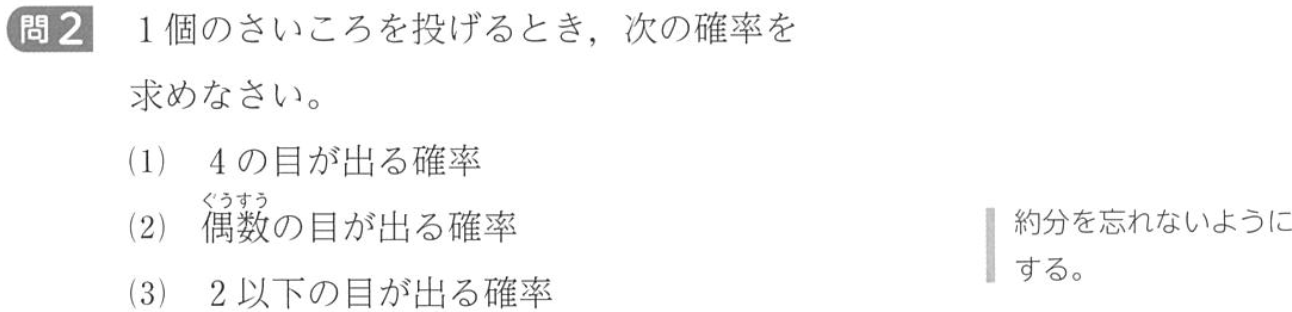
\includegraphics[height=7zw]{question2.png}
\end{figure}

\renewcommand{\thefootnote}{}
\footnotetext[1]{宿題は裏にあります.}
%注釈番号をつけないようにした

\onecolumn

{\LARGE ◎\textgt{宿題}}

\begin{figure}
  \centering
  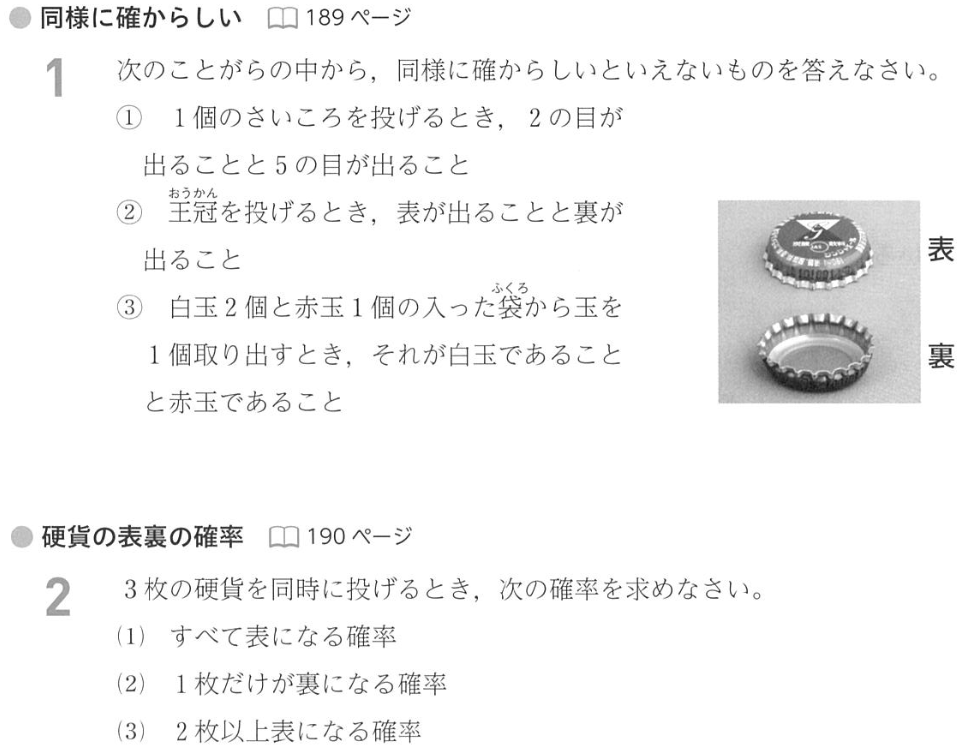
\includegraphics[height=35zw]{Homework.png}
\end{figure}

\end{document}
